\Lecture{Jayalal Sarma}{Sept 19, 2020}{06}{Catlan Bijections}{Anshu and Narasimha Sai}{$\alpha$}{JS}

\section{Introduction}
One of the classic examples to demonstrate the power of bijections is \emph{Catlan numbers}. The Catlan numbers form a sequence of natural numbers that occur in various counting problems and occurs in several seemingly different contexts. Historically, \emph{Euler} is the first person to study them. He was interested in counting the number of ways of dividing a polygon into triangles by drawing non-overlapping diagonals. Catlan numbers got their name from \emph{Eugene Catlan} when he used them to answer the \emph{Parenthesisation problem} which is the following: Consider a sequence $(a_1,a_2,\cdots,a_{n+1})$ of $n+1$ numbers, If we have to perform a binary operations $\odot$ $n$ times among them, how many number of ways are there to parenthesise (or bracket) them using $n$ parenthesis of single type (say $'()'$). In this lecture, we will see a few equivalent problems to this and then arrive at an explicit expression of Catlan numbers.
\section{Equivalent Bijections}
In this section, we see a few equivalent problems of the \emph{parenthesisation} problem and argue that answer to each of them is also the \emph{catlan number}
\paragraph{Full binary trees} If we observe the Parenthesisation problem carefully, we notice that every valid parentesisation of those $n+1$ numbers form a \emph{full binary tree} (a binary tree in which every node have either two children or no children) of $n+1$ leaves and $n$ internal nodes where leaves represents the numbers $a_1,\cdots,a_{n+1}$ and each internal node corresponds to one operation. Therefore, there's an implicit bijection between the set of valid parenthesisations and full binary trees with $n$ internal nodes. Therefore, 
\begin{equation}
    \substack{\textrm{number of valid parenthesisations of }\\ n+1 \textrm{ elements }}  = \substack{\textrm{number of full binary trees with }\\ n \textrm{ internal nodes}}
\end{equation}  

\paragraph{Balanced parenthesised strings} A balanced parenthesised string of length $2n$ is a string consists of $n$ left brackets $'('$ and $n$ right brackets $')'$ in which every prefix of the string has number of left brackets $'('$ $\geq$ number of right brackets $')'$. One can easily observe the bijection from set of balanced paranthesised string to valid parenthesisations of $n+1$ numbers

\paragraph{Euler's problem} Find the number of ways of triangulating a polygon with $n+2$ edges

\paragraph{Handshaking problem} Consider a scenario where $2n$ people are sitting around a table. How many ways they can shake hands with each other without crossing hands. We leave it as an exercise to establish bijections from \emph{Euler's} problem to \emph{Full binary tree} problem and \emph{handshaking} problem to \emph{balanced parenthesised strings} problem.
\jsay{Establish bijections from \emph{Euler's} problem to \emph{Full binary tree} problem and \emph{handshaking} problem to \emph{balanced parenthesised strings} problem}

\section{Algebraic Expression}
In this section, we are interested in arriving at a concrete expression of the $n^{th}$ \emph{catlan number} (denoted by $c_n$). Let's solve another problem and then, by establishing a bijection to one of the above problems, we can arrive at an expression for $c_n$.

\subsection{Monotone walk on $n\times n$ grid} Suppose we have a grid of size $n\times n$. How many ways are there to go from $(0,0)$ to $(n,n)$ by using only downward edges or right edges. A sample path is represented in Fig. \ref{fig:sample-path}. We observe that each step can increment the value of exactly one of the co-ordinates by $1$. Since we have to move from $(0,0)$ to $(n,n)$, we have to increase the value of both the co-ordinates by $n$ and $n$ and thus irrespective of the path you take, the length of a path from $(0,0)$ to $(n,n)$ must be of length $n+n=2n$.

\begin{figure}[h!]
    \centering
    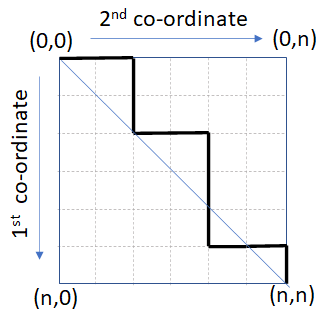
\includegraphics[width=0.4\linewidth]{images/sample-path.png}
    \caption{A path from $(0,0)$ to $(n,n)$ using downward and right edges}
    \label{fig:sample-path}
\end{figure}

If we represent each right move as $R$ and each downward move as $D$, one can observe that there's a bijection $f$ from the set of paths to set of strings of length $2n$ over the alphabet $\{D,R\}$ with number of $D$'s = number of $R$'s = $n$. Formally, if $(u_0,v_0), (u_1,v_1),\cdots,(u_{2n},v_{2n})$ represents the path where $(u_0,v_0)=(0,0)$ and $(u_{2n},v_{2n})=(n,n)$, and $b=b_1b_2\cdots b_{2n}$ represents the string where each $b_i$ is either $D$ or $R$, our bijection $f$ takes a path as input and sets $b_i$ as
$$b_i=\begin{cases}
D &\mbox{if } u_i = u_{i-1}+1\\
R &\mbox{if } v_i = v_{i-1}+1
\end{cases}$$
\begin{description}
\item \underline{Well defined:} As we have exactly $n$ $x$ co-ordinate increments and $n$ $y$ co-ordinate increments, we will have exactly $n$ $D$'s and $n$ $R$'s in our string and thus $f$ is well defined.
\item \underline{Injective:} Two different paths from $(0,0)$ to $(n,n)$ will different in at least one $(u_{i-1},v_{i-1})$ to $(u_i,v_i)$ transition where $i=1,2,\cdots,2n$, their corresponding strings under $f$ will differ in at least $i^{th}$ position and thus $f$ is injective.
\item \underline{Surjective:} Every string over $\{D,R\}$ of length $2n$ with equal number of $D$'s and $R$'s has a pre-image under $f$ which is defined by $(u_0,v_0)=(0,0)$ and $(u_i,v_i)$ is $(u_{i-1}+1,v_{i-1})$ if $b_i=R$ and $(u_{i-1},v_{i-1}+1)$ if $b_i=D$. As there will be $n$ $D$'s and $n$ $R$'s, $(u_{2n},v_{2n})=(n,n)$ and thus $f$ is surjective .
\end{description} 
Thus $f$ is bijection. As we have number of string over $\{D,R\}$ of length $2n$ with equal number of $D$'s and $R$'s equal to $\binom{2n}{n}$ (select $n$ positions out of $2n$ available and fill them with $D$'s and the rest with $R$'s). Thus the number of paths from $(0,0)$ to $(n,n)$ with only downward and rightward movements is $\binom{2n}{n}$.

Lets ask a slightly question. How many ways are there to go from $(0,0)$ to $(n+1,n-1)$ using only downward or right edges.Using a similar arguments as above, we can come up with a bijection to set of string over $\{D,R\}$ of length $2n$ with $n+1$ $D$'s and $n-1$ $R$'s. Therefore number of required paths are $\binom{2n}{n+1}=\binom{2n}{n-1}$

